\chapter{Estado del arte}\label{cap.estado}

\section{Redes neuronales para detección}
\label{sec:nets}


\subsection{Redes neuronales convolucionales}

Rigoberto Vizcay~\cite{tesis_rigoberto} se basa en redes \textit{\acrfull{cnn}} para la detección de vehículos y peatones. Una red neuronal convolucional es una red que presenta una o varias capas convolucionales. La red que implementó constaba de dos capas de convolución y dos de agrupamiento, además de la capa de salida completamente conectada. En la Figura~\ref{fig.cnn_estado_arte} se puede ver la estructura de la red.

\begin{figure}[H]
  \begin{center}
    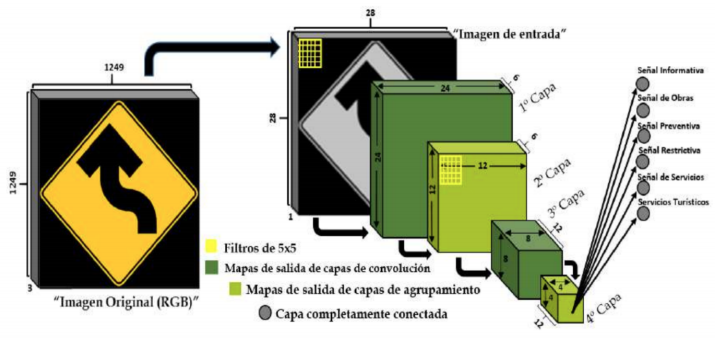
\includegraphics[width=0.7\textwidth]{figures/estado_arte/cnn.png}
		\caption{CNN Rigoberto Vizcay~\cite{tesis_rigoberto}}
		\label{fig.cnn_estado_arte}
		\end{center}
\end{figure}

Y. Abdullah, G. Mehmet, A. Iman and B. Erkan~\cite{rcnn_detection}  plantean el uso de \textit{\acrfull{rcnn}} y Faster \acrshort{rcnn} para la detección de vehículos. Por un lado, \acrshort{rcnn} para realizar las detecciones realiza tres fases que se pueden ver en la Figura~\ref{fig.rcnn}:
\begin{enumerate}
    \item Se emplea el algoritmo \textit{Selective Search}, el cual solo realiza las pruebas de detección a las regiones candidatas a tener una posible detección. Con ello se extraen aproximadamente 2000 regiones de la imagen (\textit{Region Proposal}).
    \item Se implementa una red neuronal \textit{\acrfull{cnn}} en la parte superior de cada región.
    \item Se extrapola la salida de cada \acrshort{cnn} y se ingresa en una \textit{\acrfull{svm}} para clasificar la región. Además se realiza una regresión lineal para restringir el cuadro de la detección.
\end{enumerate}

\begin{figure}[H]
  \begin{center}
    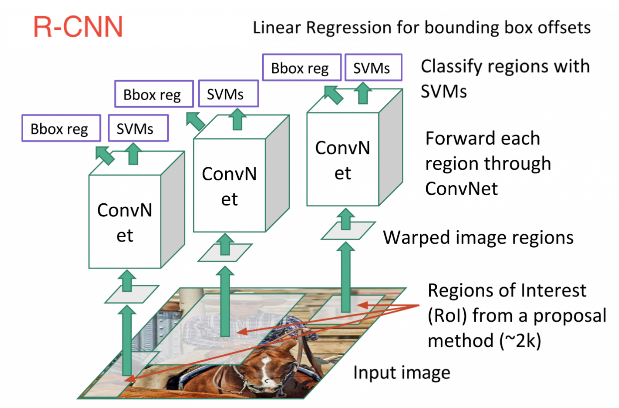
\includegraphics[width=0.7\textwidth]{figures/estado_arte/rcnn.png}
		\caption{Fases de \acrshort{rcnn}}
		\label{fig.rcnn}
		\end{center}
\end{figure}

Por otro lado, Faster \acrshort{rcnn} (Figura~\ref{fig.fast_rcnn}) es una versión más rápida que \acrshort{rcnn}, en la que se modifican algunos aspectos. En este método se incluye la técnica \textit{region proposal}, la cual determina qué regiones de la imagen tienen mayor probabilidad de contener objetos y por tanto cuáles son las regiones que se introducirán en el clasificador. Esto optimiza mucho el trabajo pues evita introducir al clasificador regiones que no sean de interés.


Ignacio Arriola~\cite{tesis_ignacio_arriola} hace también uso de Faster \acrshort{rcnn}. En este trabajo se han entrenado y comparado tres redes Faster \acrshort{rcnn} para la detección de peatones partiendo de diferentes parámetros iniciales. Con ello se pretendía estudiar la transferencia del aprendizaje, experimentando con dos redes pre-entrenadas y una inicializada con parámetros aleatorios.  Las redes pre-entrenadas se trataban de una Faster-\acrshort{rcnn}~\cite{faster_rcnn_ignacio} y una red convolucional Resnet 101 ~\cite{faster_rcnn_regnet_ignacio} como extractor de características. Cada modelo fue entrenado con una base de datos diferente (uno con \textit{\acrfull{coco}}\footnote{http://cocodataset.org/\#home} y otro con KITTI \footnote{http://www.cvlibs.net/datasets/kitti/}). Tras realizar las pruebas concluyeron que el caso que peores resultados obtenía era el que tenía valores iniciales aleatorios. También se ha analizado un caso práctico de detección de baches en carretera con los mismos modelos empleados en la detección de peatones.

\begin{figure}[H]
  \begin{center}
    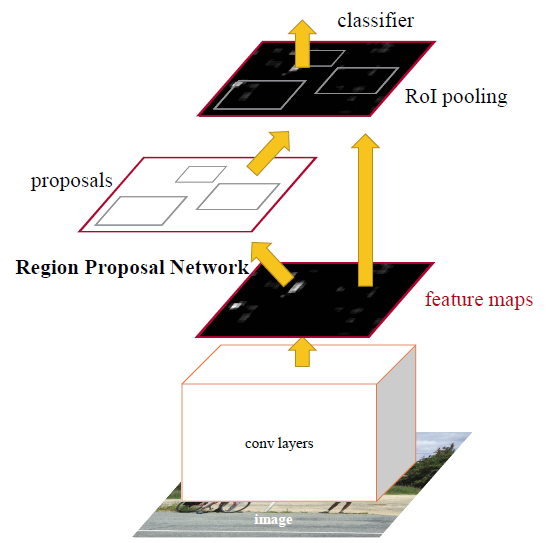
\includegraphics[width=0.5\textwidth]{figures/estado_arte/faster_rcnn.png}
		\caption{Fases de Faster \acrshort{rcnn}}
		\label{fig.fast_rcnn}
		\end{center}
\end{figure}

\section{Bases de datos de detección}
La detección de personas pretenden encontrar una persona en una imagen o en un vídeo. Dado que queremos encontrar la persona en cuestión bajo diferentes circunstancias, es decir, en distintos entornos y diferentes iluminaciones, necesitaremos típicamente entrenar el modelo con un conjunto de imágenes representativo. Por este motivo, a lo largo de los últimos años han surgido en la comunidad internacional diferentes \textit{datasets} con el fin de solucionar este problema.

\subsection{\acrfull{coco}}
El \textit{dataset} de \acrfull{coco}\footnote{\url{https://cocodataset.org}}\cite{cocodataset} es uno de los conjuntos de imágenes mas usados para entrenar redes para detección de objetos. Esto se debe a que contiene mas de 200.000 imágenes etiquetadas\ref{fig.coco} con en torno a 80 clases de objetos diferentes. Además no solo se usa para detección, sino, para segmentación, clasificación y otros usos.

\begin{figure}[H]
  \begin{center}
    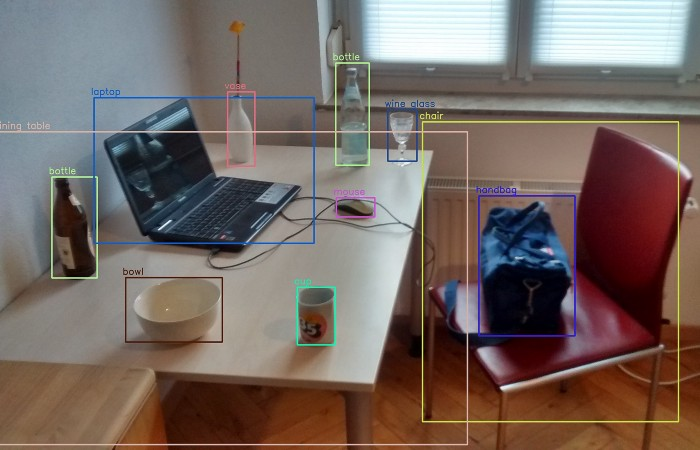
\includegraphics[width=0.5\textwidth]{figures/estado_arte/coco.jpeg}
		\caption{ejemplo de \textit{\acrshort{coco}}}
		\label{fig.coco}
		\end{center}
\end{figure}

\subsection{Open Images}
\textit{Open Images}\footnote{\url{https://storage.googleapis.com/openimages/web/index.html}}~\cite{OpenImages} es un conjunto de datos de aproximadamente 9 millones de imágenes anotadas(figura \ref{fig.oi}) con etiquetas de nivel de imagen, cajas delimitadoras de objetos, máscaras de segmentación de objetos, relaciones visuales y narraciones localizadas. Las cajas han sido dibujadas en gran parte manualmente por anotadores profesionales para garantizar la precisión y la coherencia. Las imágenes son muy diversas y a menudo contienen escenas complejas con varios objeto. 

También ofrece anotaciones de relaciones visuales, indicando pares de objetos en relaciones particulares (por ejemplo, "mujer tocando la guitarra"), propiedades de los objetos (por ejemplo, "la mesa es de madera") y acciones humanas (por ejemplo, "la mujer está saltando").

\begin{figure}[H]
  \begin{center}
    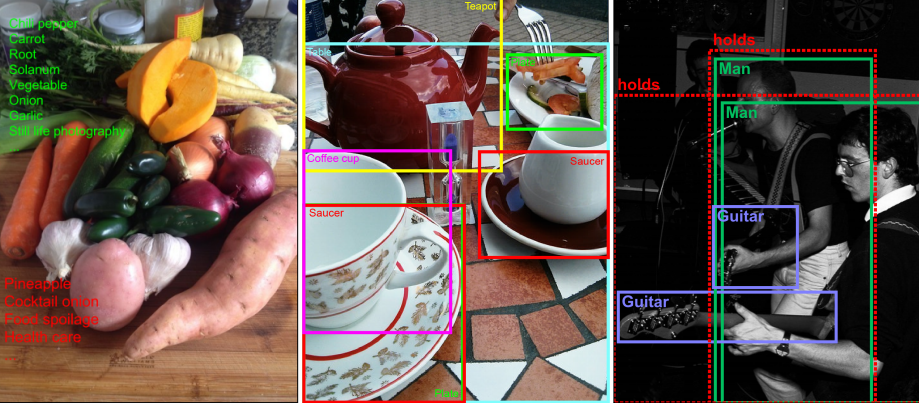
\includegraphics[width=0.5\textwidth]{figures/estado_arte/openImages.png}
		\caption{ejemplo de \textit{Open Images}}
		\label{fig.oi}
		\end{center}
\end{figure}

\subsection{\acrfull{voc} 2012}

Este conjunto de datos contiene los datos del \textit{\acrfull{voc}} 2012\footnote{\url{http://host.robots.ox.ac.uk/pascal/VOC/voc2012/}}~\cite{pascal-voc-2012}, también conocido como \textit{VOC2012}, correspondiente a las competiciones de Clasificación y Detección. Un total de 11540 imágenes están incluidas en este conjunto de datos, donde cada imagen contiene un conjunto de objetos, de 20 clases diferentes, haciendo un total de 27450 objetos anotados.